\documentclass[conference]{IEEEtran}
\IEEEoverridecommandlockouts
% The preceding line is only needed to identify funding in the first footnote. If that is unneeded, please comment it out.
\usepackage{cite}
\usepackage{amsmath,amssymb,amsfonts}
\usepackage{algorithmic}
\usepackage{graphicx}
\usepackage{textcomp}
\usepackage{xcolor}
\usepackage{float}
\usepackage{multirow}
\usepackage{multicol}

\usepackage[table]{xcolor}
\usepackage{colortbl}



\def\BibTeX{{\rm B\kern-.05em{\sc i\kern-.025em b}\kern-.08em
    T\kern-.1667em\lower.7ex\hbox{E}\kern-.125emX}}

\makeatletter
\newcommand{\linebreakand}{%
  \end{@IEEEauthorhalign}
  \hfill\mbox{}\par
  \mbox{}\hfill\begin{@IEEEauthorhalign}
}


\begin{document}



\title{FORECASTING TECH STOCKS: STATISTICAL, MACHINE LEARNING, AND DEEP LEARNING APPROACHES
}


\author{
  \IEEEauthorblockN{1\textsuperscript{st} NGUYEN SY LE HOANG}
  \IEEEauthorblockA{\textit{University of Information Technology} \\
    Ho Chi Minh City, Vietnam \\
    21520870@gm.uit.edu.vn}
  \and
        \IEEEauthorblockN{2\textsuperscript{nd} NGUYEN NGOC BINH}
  \IEEEauthorblockA{\textit{University of Information Technology} \\
    Ho Chi Minh City, Vietnam \\
    21521876@gm.uit.edu.vn}

  \and
  \IEEEauthorblockN{3\textsuperscript{rd} NGUYEN LY DANG KHOA}
  \IEEEauthorblockA{\textit{University of Information Technology} \\
    Ho Chi Minh City, Vietnam \\
    21522229@gm.uit.edu.vn}
  \linebreakand % <------------- \and with a line-break

  \IEEEauthorblockN{4\textsuperscript{th} NGUYEN BA HAO}
  \IEEEauthorblockA{\textit{University of Information Technology} \\
    Ho Chi Minh City, Vietnam \\
    21520827@gm.uit.edu.vn}
  \and
  \IEEEauthorblockN{5\textsuperscript{th} HO VAN VINH}
  \IEEEauthorblockA{\textit{University of Information Technology} \\
    Ho Chi Minh City, Vietnam \\
    21520530@gm.uit.edu.vn}
}


\maketitle

\begin{abstract}
The prediction of stock prices is a challenging task due to the complexity and volatility of the financial market. This has led to a growing interest in using machine learning methods to improve the accuracy of stock price forecasting. In this paper, we compare the performance of 10 different approaches, including Linear Regression, ARIMA, RNN, GRU, LSTM, SARIMAX, Boosting Model, Stacking Model, ResNet, and CNN-LSTM, in predicting stock prices. Three Vietnamese tech stock market datasets, ELC, CMG, and FPT, are used for evaluation. The performance of each model is analyzed and compared in detail to identify the most reliable and accurate method for stock price prediction. 
\end{abstract}

\begin{IEEEkeywords}
Stock, Linear Regression, ARIMA, RNN, GRU, LSTM, SARIMAX, Boosting Model, Stacking Model, ResNet, CNN-LSTM
\end{IEEEkeywords}

\section{INTRODUCTION}
This research focuses on exploring and applying various machine learning models for stock price prediction. The models investigated in this study include Linear Regression, ARIMA, RNN, GRU, LSTM, SARIMAX, Boosting Model, Stacking Model, ResNet, and CNN-LSTM.

In the investment and finance domain, accurate stock price prediction is crucial for making informed trading decisions. While traditional methods like fundamental and technical analysis have been employed, the emergence of machine learning techniques has opened doors for improved and more precise forecasting.

It's important to note that each machine learning model has its unique characteristics and operation methods, encompassing data preprocessing, model building, optimization techniques, and performance evaluation. This paper will delve deeper into these models and assess their effectiveness in stock price prediction.

The objective of this research is to evaluate and compare the strengths, weaknesses, and performance of the aforementioned models. We will examine their flexibility and adaptability to stock market data. Their capability for high-accuracy forecasting, especially under volatile and uncertain market conditions, and their ability to handle time-related factors and data correlations will also be explored.

By conducting a comprehensive analysis and comparison of these machine learning models, this research aims to elevate the accuracy of stock price predictions and support informed decision-making in the investment and finance sector.

\section{RELATED WORKS}

In recent years, there has been a substantial amount of research dedicated to predicting stock prices using various machine learning, statistical models and deep learning models.

Ziyue Yu et al., 2024 \cite{arima} investigates the application of the ARIMA model for stock price prediction using real data from the China Stock Market and Accounting Research Database (CSMAR) and statistical software SPSS. The study explores the potential of ARIMA in identifying trends but also acknowledges limitations due to the model's inherent simplicity when applied to complex financial markets

Birari et al., 2024 \cite{sarimax} employs SARIMAX to analyze the closing prices of the IT Index. The model incorporates technical indicators like moving averages and RSI to enhance prediction accuracy. The study reveals a significant influence of price volatility (difference between high and low) and the 14-day moving average on the index' closing price. This highlights the potential of SARIMAX for financial analysis and decision-making, considering both internal (time series) and external factors.

Gupta et al., 2019 \cite{linear} demonstrate the effectiveness of linear regression in stock price prediction. Utilizing historical stock price data and relevant features as independent variables, they apply linear and support vector regression to forecast Google's stock price. This highlights the applicability of linear regression as a fundamental yet robust method for stock price prediction.

Regarding the application of Boosting Models, the two most commonly used models are AdaBoost (Adaptive Boosting) and Gradient Boosting Machines (GBM). Rebwar M. Nabi et al., 2020 \cite{adaboost} applied these models to compare the classifying accuracy rates of boosting models with other classifiers. Minjae Park et al., 2019 \cite{gbm} applied GBM combined with Feature Engineering (GBM-wFE) to predict stock prices with a more promising accuracy rate compared to previous approaches.

Zi Ye et al., 2022 \cite{stacking} have published a paper utilizing a stacking ensemble model combining GRU and LSTM to predict Bitcoin prices using price data, technical indicators, and sentiment indexes from Twitter comments on Bitcoin.

Yongqiong Zhu et al., 2020 \cite{rnn} employed Recurrent Neural Networks (RNNs) to predict Apple's stock price using ten years of historical data. Their model achieved an impressive 95\% accuracy with a minimal error of 0.1\%. This highlights the effectiveness of RNNs in capturing complex patterns and sequences in stock market data, leading to accurate price predictions. 

Sidra Mehtab et al., 2021 \cite{lstm}  proposed using market data to predict stock prices using machine learning techniques such as recurrent neural networks (RNNs), in the form of Long Short-Term Memory (LSTMs), and in which the weights are adjusted for each data point using the stochastic gradient descent (SGD) algorithm

Yagao et al. 2021 \cite{gru} employed Gated Recurrent Units (GRUs) and optimized them using the LASSO dimensionality reduction method. Their approach demonstrated remarkable effectiveness in predicting the SSE Composite Index, encompassing all stocks traded on the Shanghai Stock Exchange (SSE), from 2007 to 2021.

Yuanzhe Jia et al. 2020 \cite{resnet} employed a ResNet architecture to extract features for identifying dependencies between stock prices across time windows. These features were then integrated into an LSTM model to assist clients in risk mitigation and profit generation within the stock market.

Yushi Guan et al. 2020 \cite{cnnlstm} have proposed a combined CNN-LSTM model for predicting stock prices without the need for additional input data such as technical and economic indicators. The proposed model outperforms simple LSTM models as well as non-neural methods such as RF, KNN, and linear regression.

\section{MATERIALS}
\subsection{DATASET}

This study analyzes stock trends in Vietnam's technology sector. We focus on three companies: FPT Corporation   , Elcom Technology Communications Corp, and CMC Corporation. Data encompassing the period from March 26th, 2018, to March 22th, 2024, was obtained from Investing.com. Each initial dataset included approximately 1500 data points with seven attributes: Date, Close Price, Open Price, High Price, Low Price, Trading Volume, and Change. 


\subsection{DESCRIPTIVE STATISTICS}
\begin{table}[H]
  \centering
  \caption{FPT, ELC, CMC’s Descriptive Statistics}
\begin{tabular}{|>{\columncolor{red!20}}c|c|c|c|}
    \hline
     \rowcolor{red!20} & FPT & ELC & CMC \\ \hline
     Count & 1500 & 1499 & 1500 \\ \hline
     Mean & 56116.29 & 11376.6 & 33577.43
\\ \hline
     Std & 27352.61 & 6489.9 & 12445.16
\\ \hline
     Min &19765.8 & 3409 & 12353.9
\\ \hline
     25\% & 30228.82 & 5666.7 & 23816.97
\\ \hline
     50\% & 55109 & 9465 & 30039\\ \hline
     75\% & 80500 & 14985.45 & 44514.25
\\ \hline
     Max & 117000 & 27300 & 62430
\\ \hline
\end{tabular}
\end{table}


\begin{figure}[H]
    \centering
    \begin{minipage}{0.23\textwidth}
    \centering
    \includegraphics[width=1\textwidth]{Figure/fpt-bõ.png}
    \caption{FPT stock price's boxplot}
    \label{fig:1}
    \end{minipage}
    \hfill
    \begin{minipage}{0.23\textwidth}
    \centering
    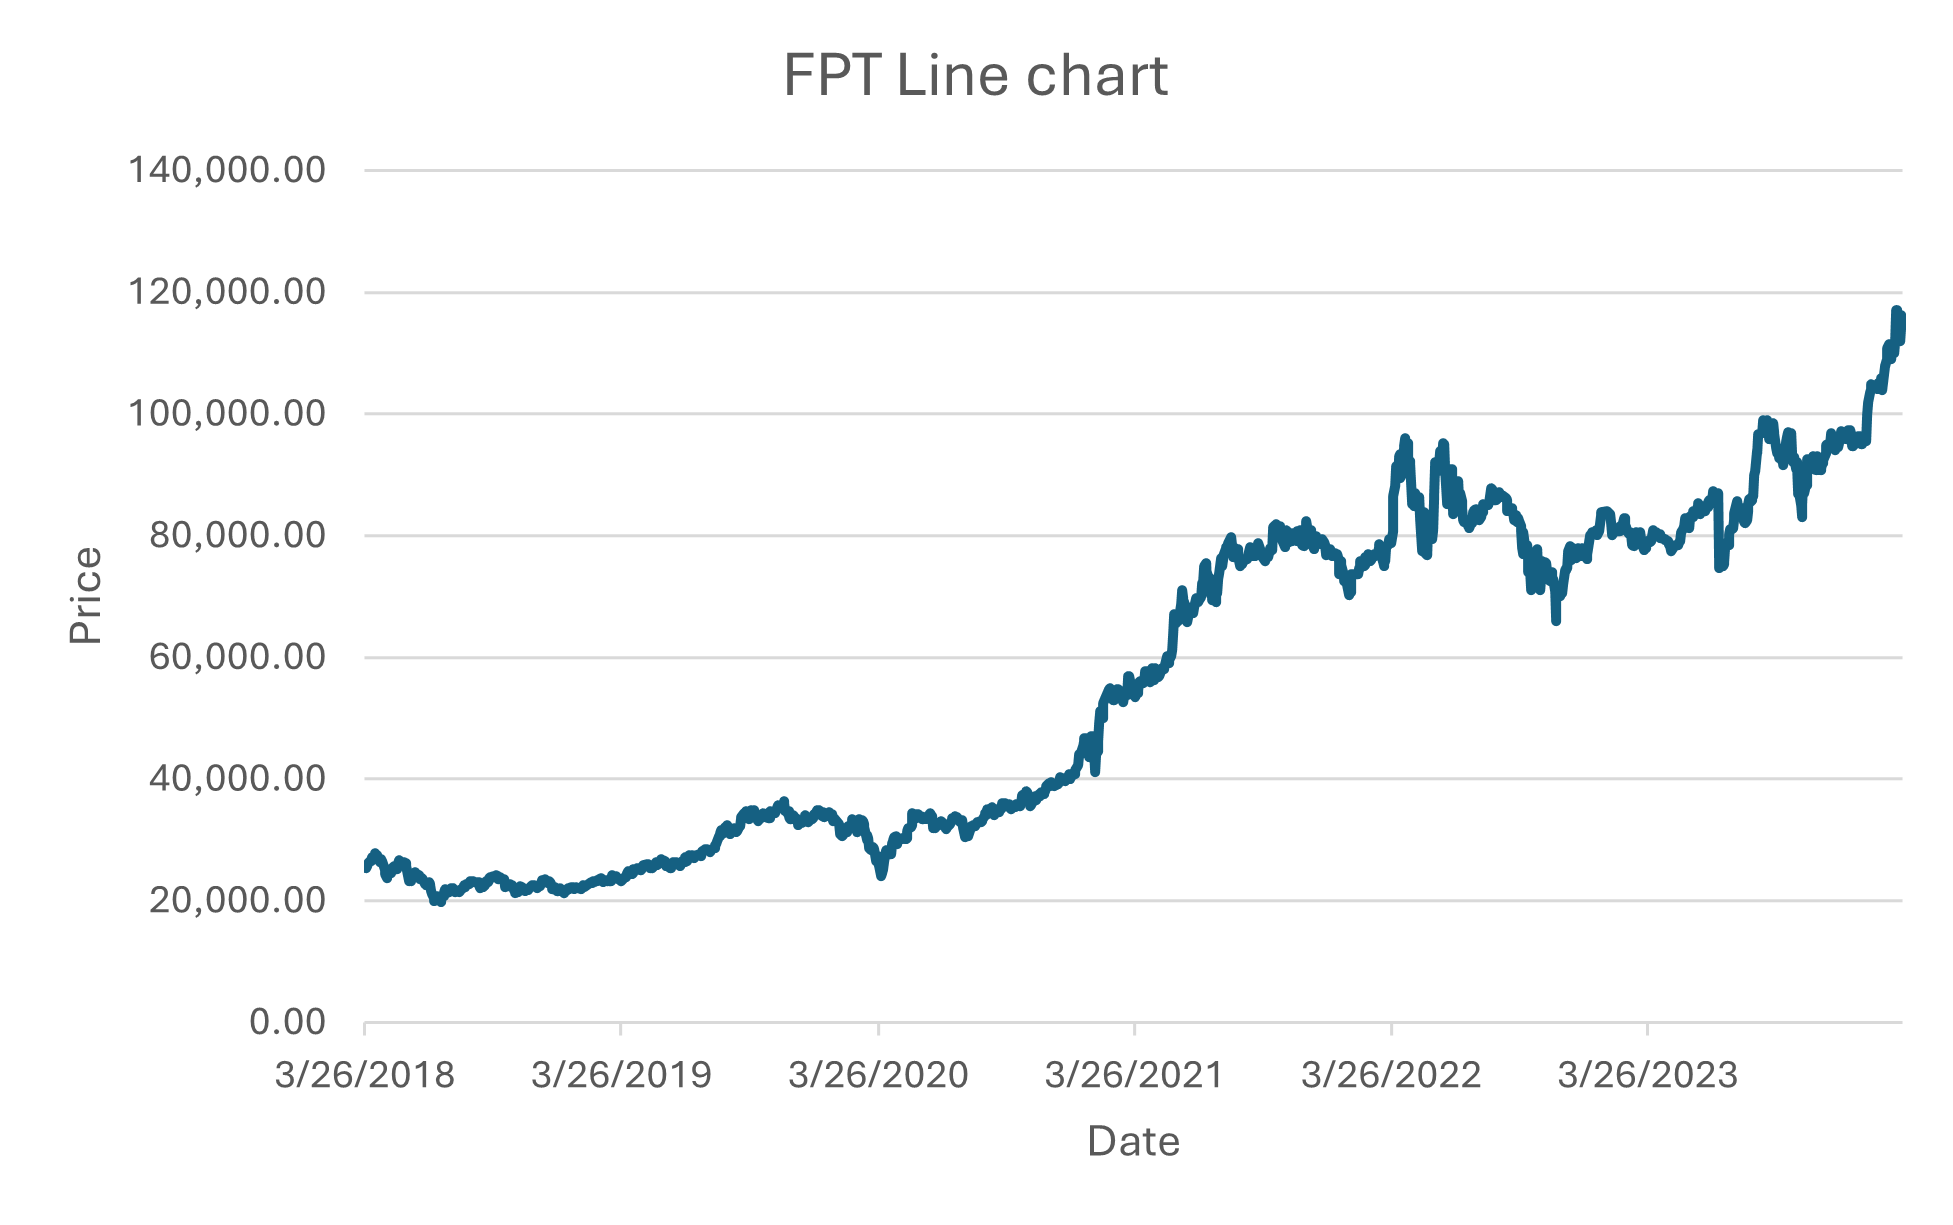
\includegraphics[width=1\textwidth]{Figure/fpt-line.png}
    \caption{FPT stock price's line chart}
    \label{fig:2}
    \end{minipage}
\end{figure}

\begin{figure}[H]
    \centering
    \begin{minipage}{0.23\textwidth}
    \centering
    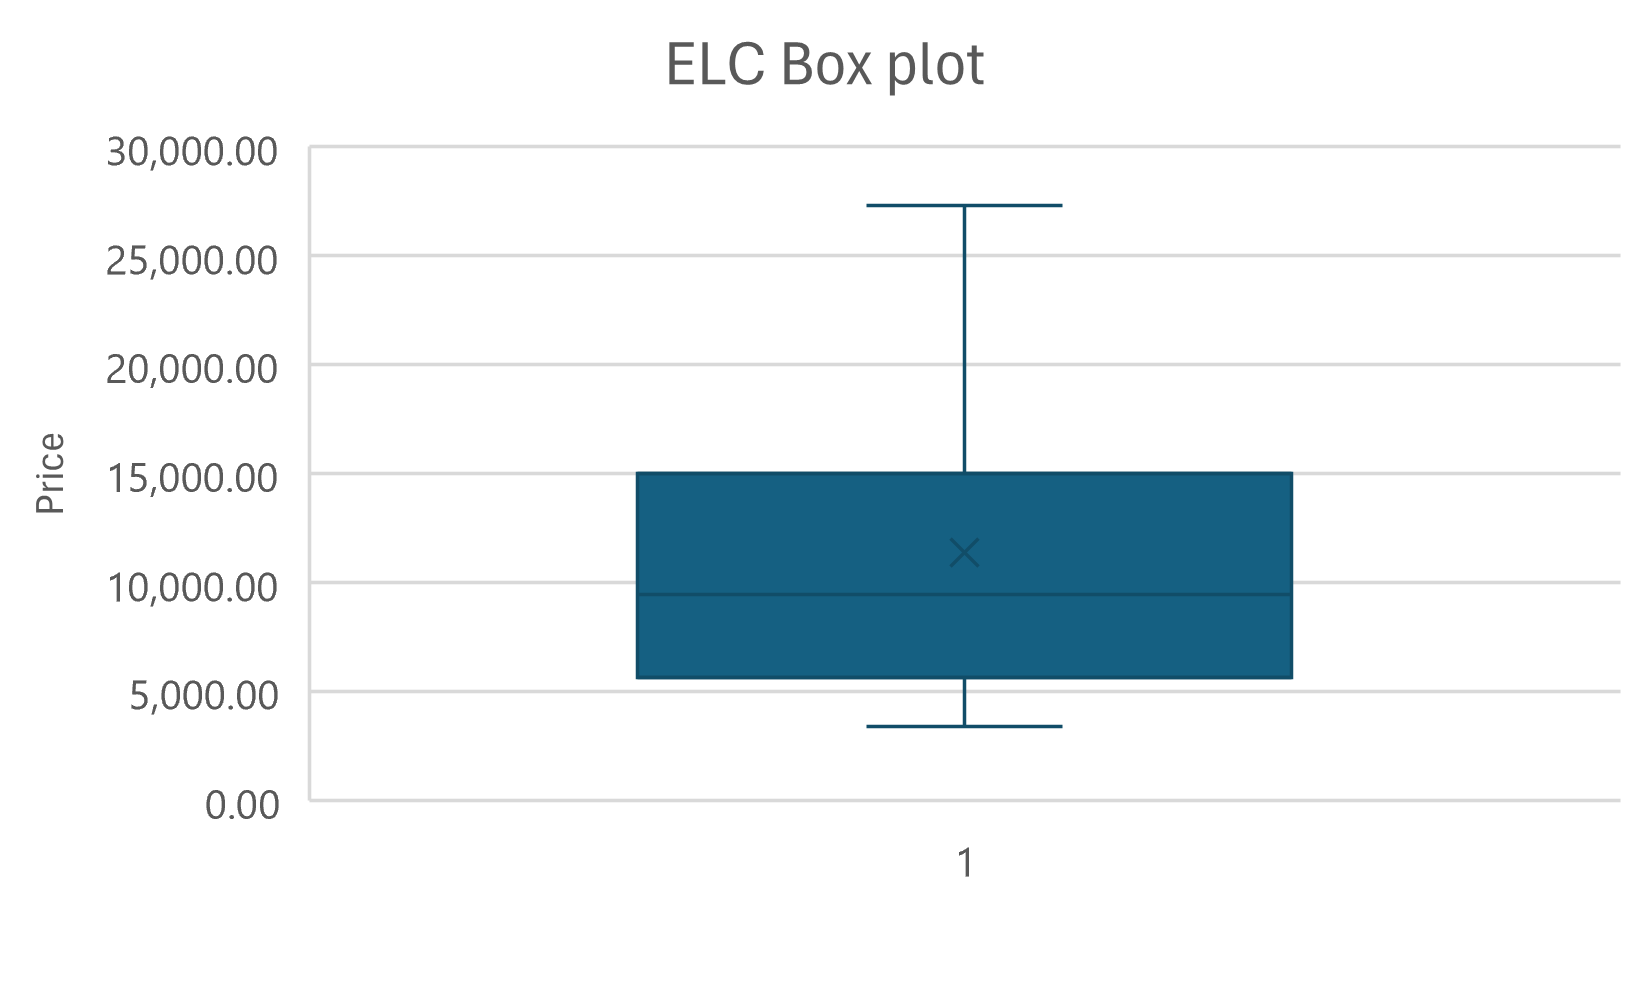
\includegraphics[width=1\textwidth]{Figure/elc-box.png}
    \caption{ELC stock price's boxplot}
    \label{fig:1}
    \end{minipage}
    \hfill
    \begin{minipage}{0.23\textwidth}
    \centering
    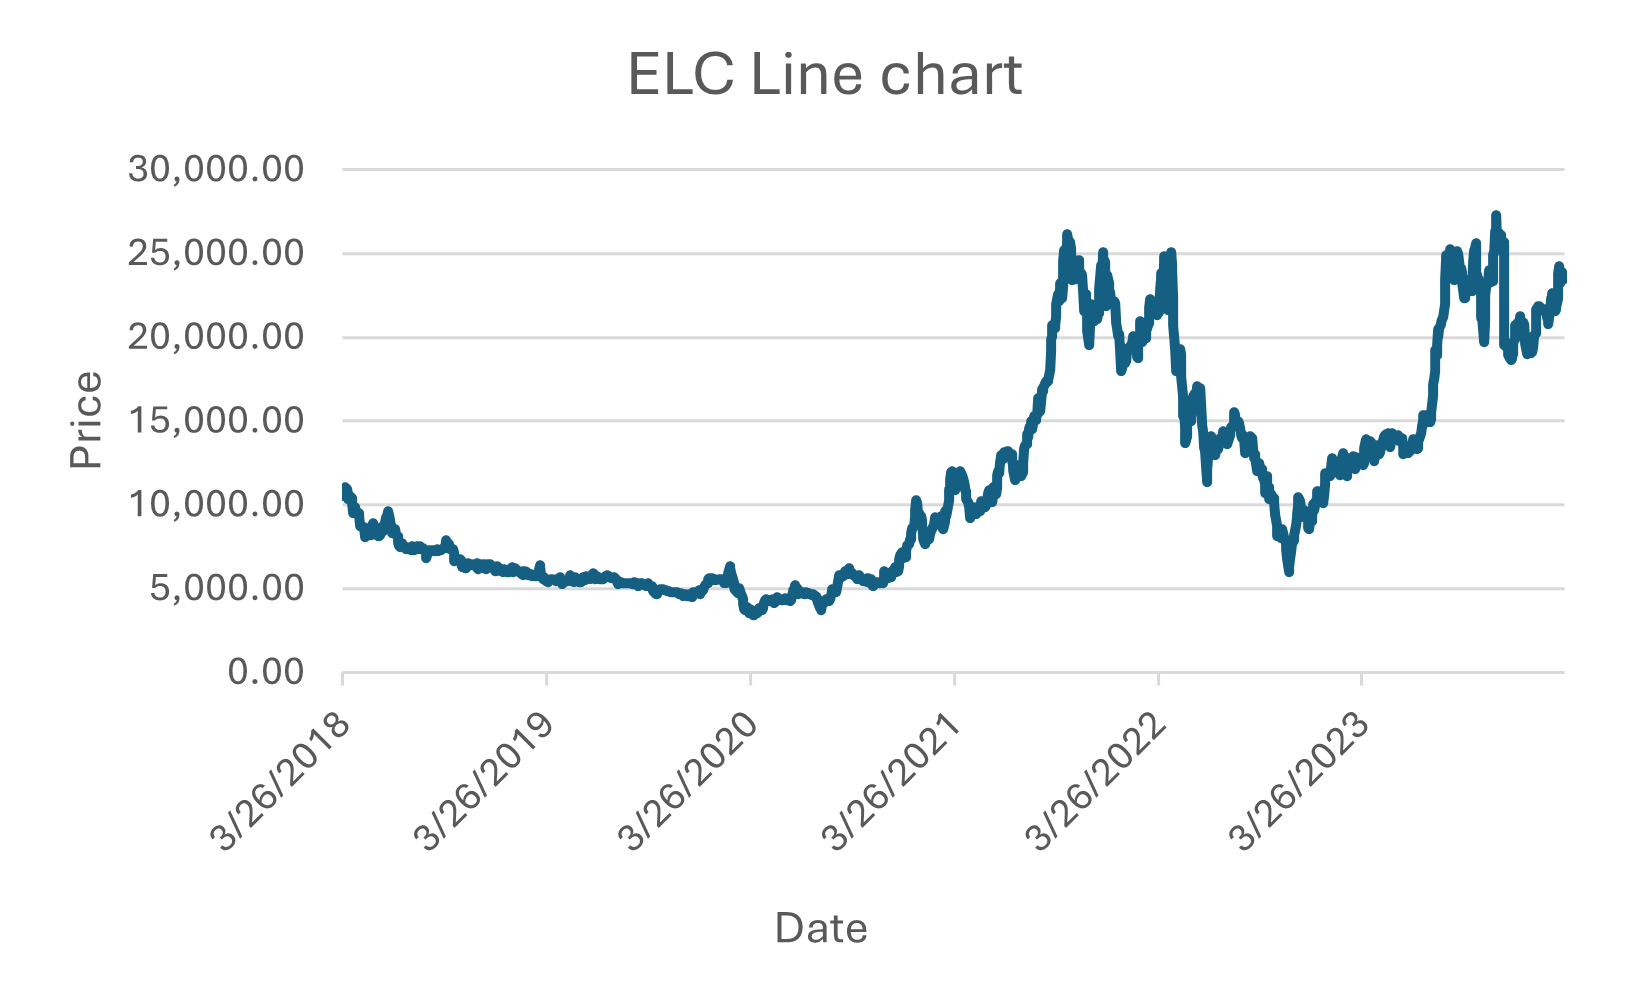
\includegraphics[width=1\textwidth]{Figure/elc-line.png}
    \caption{ELC stock price's line chart}
    \label{fig:2}
    \end{minipage}
\end{figure}

\begin{figure}[H]
    \centering
    \begin{minipage}{0.23\textwidth}
    \centering
    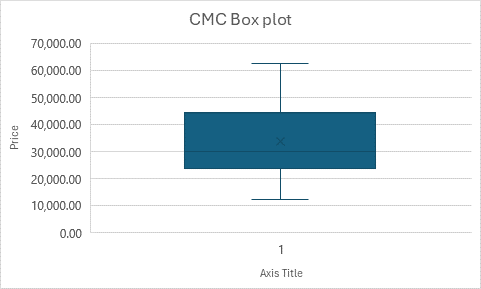
\includegraphics[width=1\textwidth]{Figure/cmcBox.png}
    \caption{CMC stock price's boxplot}
    \label{fig:1}
    \end{minipage}
    \hfill
    \begin{minipage}{0.23\textwidth}
    \centering
    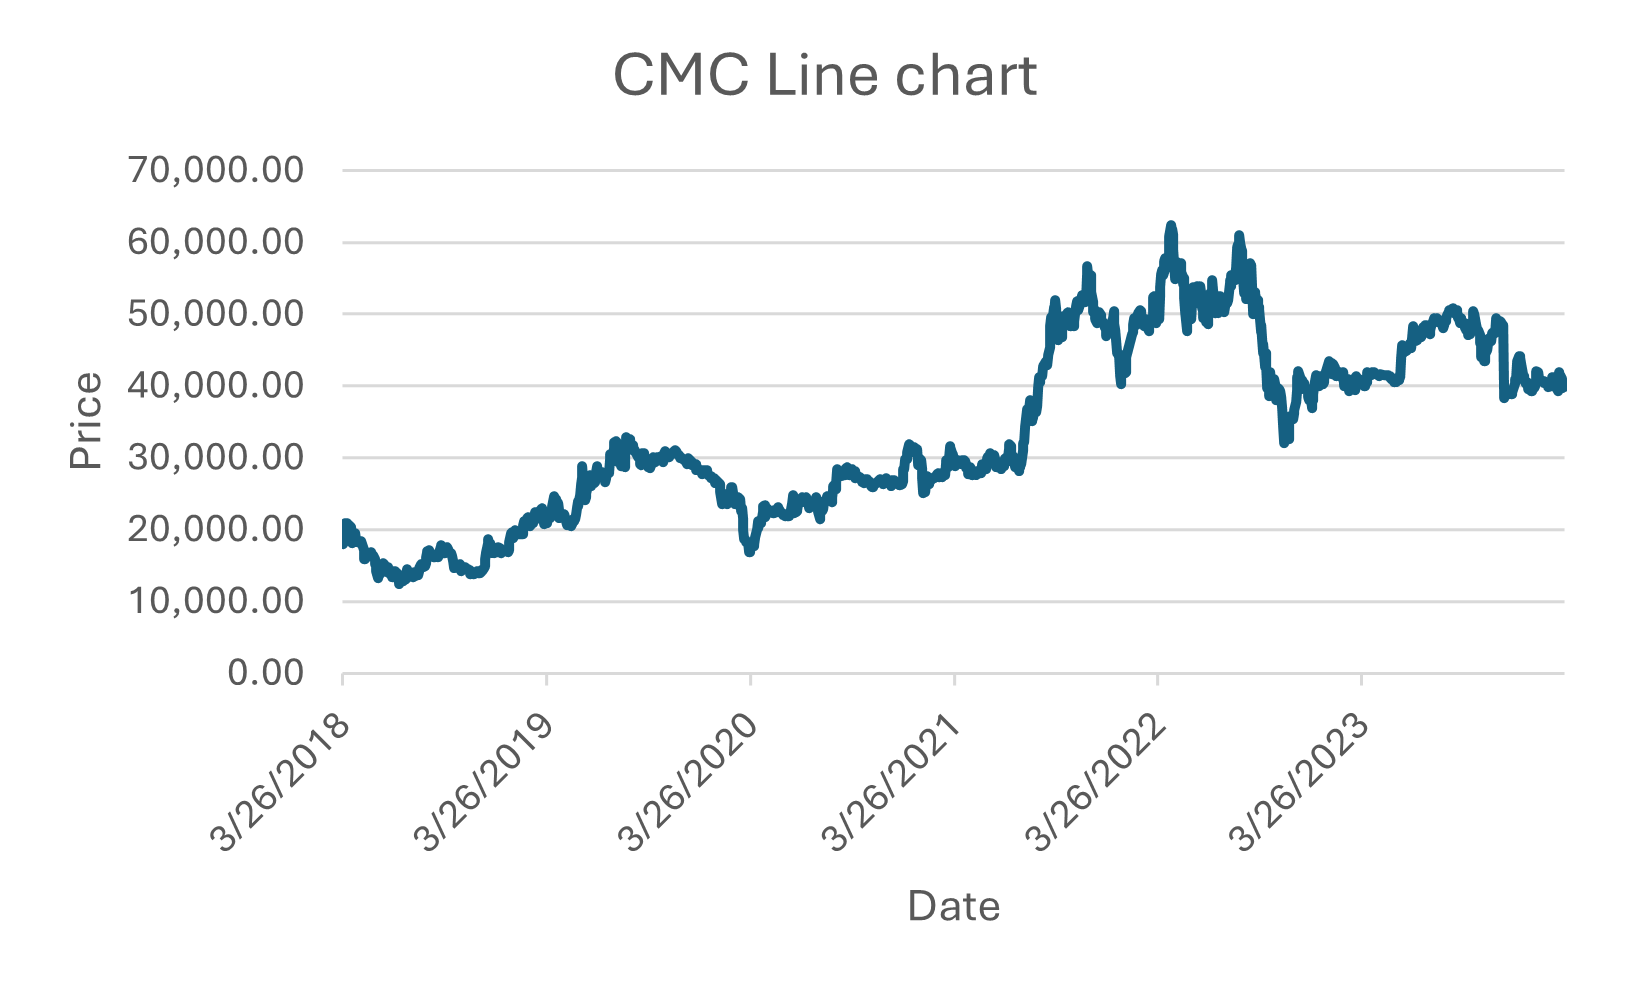
\includegraphics[width=1\textwidth]{Figure/cmc-line.png}
    \caption{CMC stock price's line chart}
    \label{fig:2}
    \end{minipage}
\end{figure}



\section{Methodology}
\subsection{Linear Regression}
Multivariable linear regression, or multiple linear regression, is a statistical method employed for examining the correlation between several independent variables (often referred to as predictors or features) and a sole dependent variable (also known as the target or response variable). This approach expands upon simple linear regression, which focuses on just one independent variable. The primary objective in multivariable linear regression is to determine the coefficients or weights that depict the linear connection between the independent variables and the dependent variable.
A multiple linear regression model has the form: 
\[Y=\beta_0+\beta_1X_1+\beta_2X_2+\cdots+\beta_kX_k+\varepsilon\]
Where:\\
	\indent\textbullet\ Y is the dependent variable (Target Variable).\\
	\indent\textbullet\ \(X_1, X_2, \ldots, X_k\) are the independent (explanatory) variables.\\
	\indent\textbullet\ \(\beta_0\) is the intercept term.\\
	\indent\textbullet\ \(\beta_1,..., \beta_k\) are the regression coefficients for the independent variables.\\
	\indent\textbullet\ \(\varepsilon\) is the error term.
 
\subsection{ARIMA}
The ARIMA model predicts future values based on its current and past value of time series data. It consists of three main components: Autoregressive (AR) component: This component captures the linear dependence of the current value on the previous values in the time series. Integrated (I) component: This component accounts for the non-stationarity in the time series by differencing the data to make it stationary and moving Average (MA) component: This component captures the linear dependence of the current value on the previous error terms. The ARIMA model is typically denoted as ARIMA (p, d, q), p is the order of the autoregressive component, d is the order of the differencing component and q is the order of the moving average component. The general form of the ARIMA (p, d, q) model can be expressed as:
\begin{align*}
Y_t = c + \phi_1 Y_{t-1} + \phi_2 Y_{t-2} + \ldots + \phi_p Y_{t-p}\\ -  \theta_1 e_{t-1} - \theta_2 e_{t-2} - \ldots - \theta_q e_{t-q} + e_t
\end{align*}
Where:
\begin{itemize}
    \item $Y_t$ is the value of the time series at time $t$.
    \item $c$ is a constant term.
    \item $\phi_1, \phi_2, \ldots, \phi_p$ are the autoregressive parameters.
    \item $\theta_1, \theta_2, \ldots, \theta_q$ are the moving average parameters.
    \item $e_t$ is the error term at time $t$.
    \item $p$ and $q$ are the orders of the autoregressive and moving average components, respectively.
\end{itemize}

\subsection{SARIMAX} 

The SARIMAX model is a time series forecasting method that considers seasonality and external factors. It incorporates ARIMA for trend and residual modeling, with additional seasonal components. The methodology involves data preprocessing, model identification through tests and decomposition, estimation with selection based on criteria, validation, and finally forecasting with visualization and interpretation. This structured approach allows for improved forecasting accuracy by incorporating both seasonal patterns and external variables. The formula for the SARIMAX model is represented as follows:
\begin{align*}
Y_t &= \beta_0 + \beta_1 X_{1,t} + \beta_2 X_{2,t} + \ldots + \beta_n X_{n,t} \\
&\quad + \phi_1 Y_{t-1} + \phi_2 Y_{t-2} + \ldots + \phi_p Y_{t-p} \\
&\quad - \theta_1 e_{t-1} - \theta_2 e_{t-2} - \ldots - \theta_q e_{t-q} + e_t
\end{align*}

Where:
\begin{itemize}
    \item $Y_t$ is the value of the time series at time $t$.
    \item $X_{1,t}, X_{2,t}, \ldots, X_{n,t}$ are exogenous variables at time $t$.
    \item $\beta_0, \beta_1, \beta_2, \ldots, \beta_n$ are the coefficients of the exogenous variables.
    \item $\phi_1, \phi_2, \ldots, \phi_p$ are the autoregressive parameters.
    \item $\theta_1, \theta_2, \ldots, \theta_q$ are the moving average parameters.
    \item $e_t$ is the error term at time $t$.
    \item $p$ and $q$ are the orders of the autoregressive and moving average components, respectively.
\end{itemize}


\subsection{Boosting Method}
Boosting operates by iteratively fitting models to the residuals of the previous models, thereby focusing on the examples that were previously misclassified or poorly predicted. This iterative process continues until a predefined stopping criterion is met, typically when the model achieves satisfactory performance or when a specified number of weak learners have been trained. The core mechanism of boosting revolves around the concept of combining multiple weak learners, often referred to as "base models" or "base classifiers," to create a strong ensemble model. In each iteration of the boosting process, a weak learner is trained on a modified version of the dataset, where instances that were misclassified in the previous iteration are given higher weights, thus emphasizing their importance in subsequent model training. Consequently, the subsequent weak learners are forced to focus on the examples that are challenging for the ensemble, gradually improving the overall predictive performance. By effectively harnessing the complementary strengths of multiple weak learners and continuously adapting to the training data, boosting algorithms are capable of producing highly accurate predictive models, making them widely utilized across various domains in machine learning. 

\begin{enumerate}
    \item \textbf{Initialize the Dataset:} Begin by initializing the dataset and assign equal weight to each of the data points.
    
    \item \textbf{Model Training:} Provide this dataset as input to the model and identify the wrongly classified data points.
    
    \item \textbf{Weight Adjustment:} Increase the weight of the wrongly classified data points.
    
    \item \textbf{Check for Required Results:} 
    \begin{itemize}
        \item If the required results are achieved, proceed to step 5.
        \item If not, return to step 2.
    \end{itemize}
    
    \item \textbf{End:} Terminate the process.
\end{enumerate}

\subsection{Stacking Method}
Stacking is a technique in machine learning where the predictions of several base models are used as input features for a meta learner, which then makes the final prediction. We can apply stacking using Support Vector Regression (SVR) and Random Forest as base models, and Ridge regression as the meta learner.
The process involves training the SVR and Random Forest models on the independent variables $x_1$, $x_2$, \ldots, $x_n$ to predict the dependent variable $y$. Then, the predictions from these base models serve as new features alongside the original independent variables. These combined features are used to train the Ridge regression model, which learns how to weigh the predictions from the base models along with the original features to make the final prediction for $y$.

\begin{figure}[htbp]
    \centering
    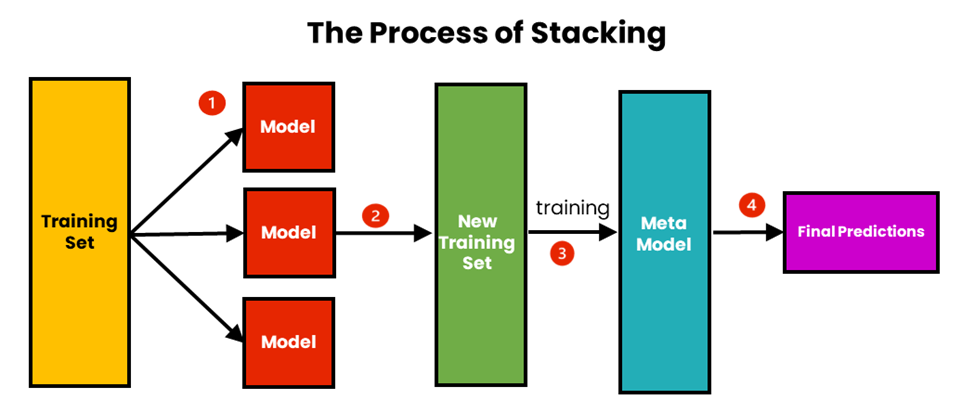
\includegraphics[width=0.5\textwidth]{Figure/stacking.png} % Adjust the width as needed
    \caption{Stacking Example}
    \label{fig:example}
\end{figure}

\subsection{Recurrent Neural Networks}
Recurrent neural networks, or RNNs, are a type of neural network that use past outputs as inputs and maintain hidden states.
\begin{figure}[htbp]
    \centering
    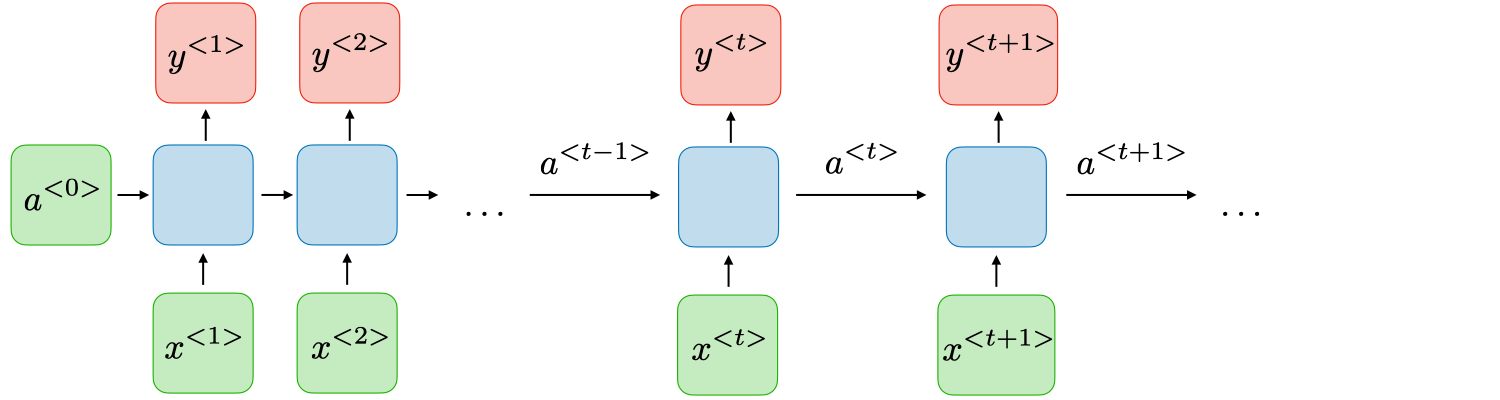
\includegraphics[width=0.5\textwidth]{Figure/architecture-rnn-ltr.png} % Adjust the width as needed
    \caption{Architecture of a traditional RNN}
    \label{fig:example}
\end{figure}

For each timestep \( t \), the activation \( a^{<t>} \) and the output \( y^{<t>} \) are expressed as follows:
\begin{align*}
a^{<t>} &= f(W_{a} \cdot x^{<t>} + U_{a} \cdot a^{<t-1>} + b_{a}) \\
y^{<t>} &= g(W_{y} \cdot a^{<t>} + b_{y})
\end{align*}

In this expression: 
\begin{itemize}
    \item \( x^{<t>} \) is the input at time \( t \).
    \item \( W_{a} \) and \( U_{a} \) are weight matrices.
    \item \( b_{a} \) and \( b_{y} \) are bias vectors.
    \item \( f \) and \( g \) are activation functions.
\end{itemize}
RNNs are widely used in various fields such as natural language processing, machine translation, speech recognition, time series prediction, and many other applications involving sequential data.

\subsection{Long Short-Term Memory}
Long Short-Term Memory (LSTM) is a variety of RNN designed to address the vanishing gradient problem found in traditional RNNs. It excels at learning long-term dependencies, especially in sequence prediction tasks.
LSTMs are structured as a chain of repeating modules of neural networks, with each module containing four neural network layers. 
\begin{figure}[htbp]
    \centering
    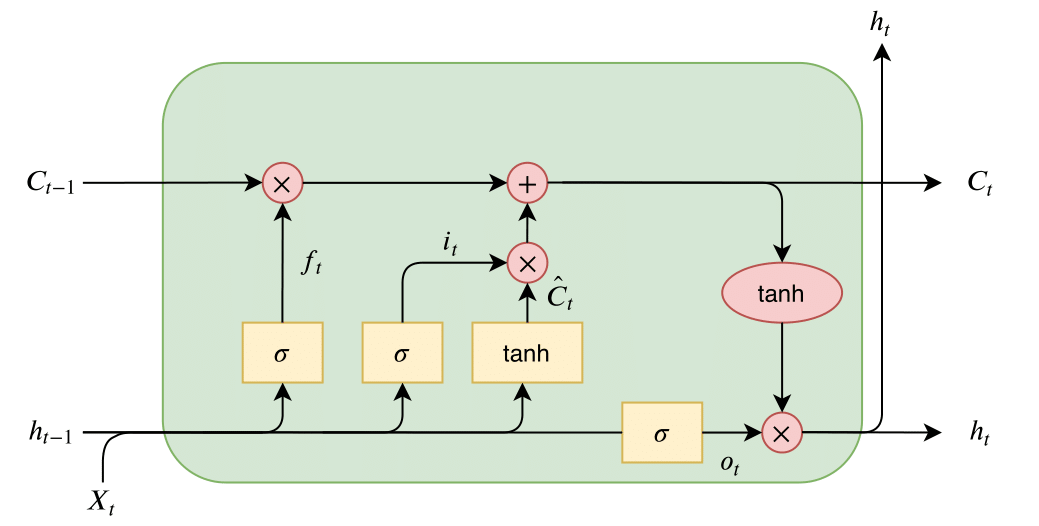
\includegraphics[width=0.5\textwidth]{Figure/lstm.png} % Adjust the width as needed
    \caption{Architecture of a LSTM module}
    \label{fig:example}
\end{figure}

LSTMs introduce memory cells that can retain information over long sequences. Each memory cell comprises three key components: an input gate, a forget gate, and an output gate. These gates help protect and regulate the cell state.

\vspace{4}
\textbf{Forget gate:} Utilizes a sigmoid layer to determine which information should be discarded from the cell state.
\[
f_t = \sigma(W_f [h_{t-1}, x_t] + b_f)
\]

\textbf{Input gate:} Determines what new information should be stored in the cell state. It includes two parts: a sigmoid layer (which decides which values to update) and a tanh layer (which creates a vector of new candidate values to add to the cell state).
\[
i_t = \sigma(W_i [h_{t-1}, x_t] + b_i)
\]
\[
\tilde{C}_t = \tanh(W_C [h_{t-1}, x_t] + b_C)
\]

\textbf{Update Cell State:} The cell state is updated by combining the old cell state, scaled by the forget gate, and the new candidate values, scaled by the input gate.
\[
C_t = f_t * C_{t-1} + i_t * \tilde{C}_t
\]

\textbf{Output gate:} Filters the information that the LSTM will output based on the updated cell state. It includes a sigmoid layer and a tanh function.
\[
o_t = \sigma(W_o [h_{t-1}, x_t] + b_o)
\]
\[
h_t = o_t * \tanh(C_t)
\]

\subsection{Gated Recurrent Unit}
The internal structure of GRU is simpler as compared to the LSTM and is easier to train as fewer computations are involved. These simplifications are achieved primarily in two
ways: The input and the forget gates are combined into a single gate referred to as the update gate. The internal/cell state and the hidden state are merged.

\begin{figure}[htbp]
    \centering
    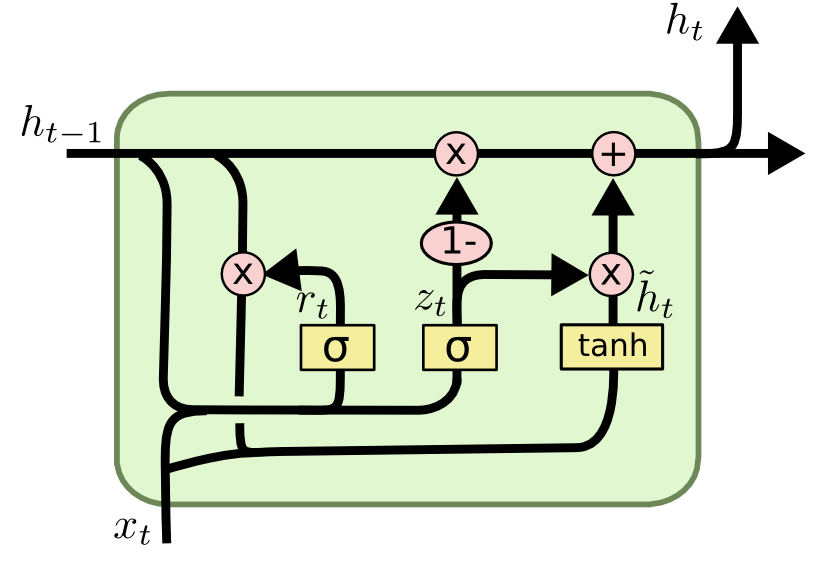
\includegraphics[width=0.5\textwidth]{Figure/GRU.png} % Adjust the width as needed
    \caption{Architecture of a GRU module}
    \label{fig:example}
\end{figure}


\textbf{Update Gate:} \quad
z_t &= \sigma(W_z \cdot [h_{t-1}, x_t]) \\

\textbf{Reset Gate:} \quad
r_t &= \sigma(W_r \cdot [h_{t-1}, x_t]) \\

\textbf{Candidate Hidden State:} \quad
\overline{h}_t &= \tanh(W \cdot [r_t \circ h_{t-1}, x_t]) \\

\textbf{Final Hidden State:} \quad
h_t &= (1 - z_t) \circ h_{t-1} + z_t \circ \hat{h}_t


\subsection{CNN-LSTM}
CNN-LSTM is a hybrid deep learning model that combines Convolutional Neural Networks (CNNs) and Long Short-Term Memory (LSTM) networks. This combination leverages the strengths of both architectures to handle data with spatial and temporal dependencies.

\begin{figure}[htbp]
    \centering
    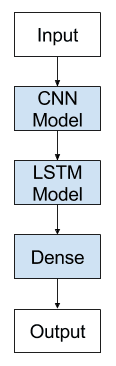
\includegraphics[height=0.3\textheight]{Figure/cnnlstm.png} % Adjust the width and height as needed
    \caption{Architecture of a CNN-LSTM model}
    \label{fig:example}
\end{figure}

The CNN-LSTM model consists of two main components:

\textbf{CNN Model:} This component is responsible for extracting spatial features from the input data. It applies convolutional layers to capture local patterns and uses pooling layers to reduce the spatial dimensions while retaining important information. The output of the CNN model is a set of learned features, which represent the spatial characteristics of the input data.

\textbf{LSTM Model:} This component takes the learned features from the CNN model as input and processes them over time. The LSTM model utilizes recurrent connections and memory cells to capture long-term dependencies and relationships between data points. Unlike standard RNNs, LSTMs are equipped with gating mechanisms that help them maintain and update information over long sequences, making them particularly effective in handling temporal dependencies.

\subsection{Residual neural network}
In traditional deep neural networks, the vanishing gradient problem occurs when gradients become very small as they propagate through many layers, leading to slower learning or complete failure in very deep architectures. ResNets solve this by using skip connections, or residual connections, which allow gradients to bypass certain layers.

\begin{figure}[htbp]
    \centering
    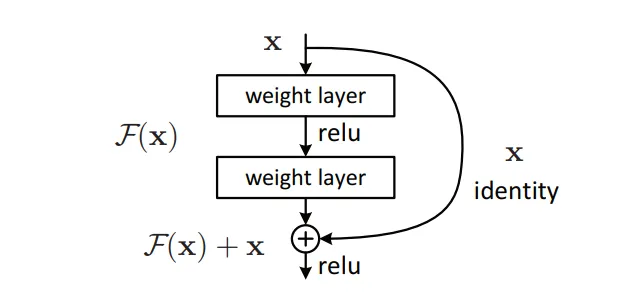
\includegraphics[width=0.5\textwidth]{Figure/resnet.png}
    \caption{Skip connection}
    \label{fig:enter-label}
\end{figure}

The architecture of ResNet is based on a series of residual blocks. Each residual block consists of multiple convolutional layers with a skip connection, also known as a shortcut or identity connection. The residual block can be represented as follows:
\begin{figure}[htbp]
    \centering
    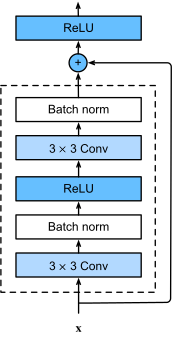
\includegraphics[height=0.3\textheight]{Figure/resnet-block.png}
    \caption{A residual block}
    \label{fig:enter-label}
\end{figure}

\section{RESULT}

\subsection{Evaluation Methods}
\textbf{Mean Percentage Absolute Error} (MAPE): is the average percentage error in a set of predicted values.\\
\begin{align*}
    MAPE=\frac{100\%}{n}  \sum_{i=1}^{n} |y_i-\hat{y_i} |  = 1 
\end{align*}

\textbf{Root Mean Squared Error} (RMSE): is the square root of average value of squared error in a set of predicted values.\\
\begin{align*}
RMSE=\sqrt{\sum_{i=1}^{n} \frac{(\hat{y_i}-y_i )^2}{n} }
\end{align*}

\textbf{Mean Absolute Error} (MAE): is the average of the absolute differences between the actual and predicted values.
\begin{align*}
MAE = \frac{1}{n} \sum_{i=1}^{n} \left| y_i - \hat{y_i} \right| 
\end{align*}

Where: \\
	\indent\textbullet\ \(n\) is the number of observations in the dataset.\\
	\indent\textbullet\ \(y_i\)  is the true value.\\
	\indent\textbullet\ \(\hat{y_i}\) is the predicted value.

\subsection{Evaluation} 

\begin{table}[H]
    \centering
    \caption{fpt dataset's evaluation}
    \begin{tabular}{|c|c|c|c|c|}
 \hline
 \rule{0pt}{2ex}
 \centering Model & Ratio & RMSE & MAPE (\%) & MAE\\
 \hline
 \multirow{3}{*}{Linear} & 7:3 & 9187.284 & 9.861 & 8202.381 \\ 
 & 8:2 & 8625.273 & 8.969 & 7645.923 \\ 
 & \textbf{9:1} & \textbf{5506.758} & \textbf{4.316} & \textbf{4276.720} \\
 \hline
 \multirow{3}{*}{Arima} & 7:3 & 19078.233 & 21.493 & 17859.367 \\ 
 & \textbf{8:2} & \textbf{6490.282} & \textbf{5.071} & \textbf{4736.232} \\ 
 & 9:1 & 10585.769 & 8.958 & 8995.129 \\
 \hline
 \multirow{3}{*}{Sarimax} & 7:3 & 11096.746 & 11.551 & 9564.850 \\ 
 & \textbf{8:2} & \textbf{13021.292} & \textbf{9.839} & \textbf{9531.102} \\ 
 & 9:1 & 14302.654 & 12.431 & 12465.231 \\
 \hline
 \multirow{3}{*}{Boosting} & 7:3 & 9330.21 & 10 & 8342.168 \\ 
 & 8:2 & 9375.80 & 9.9 & 8403.87 \\ 
 & \textbf{9:1} & \textbf{6669.22} & \textbf{4.8} & \textbf{4834.467} \\
 \hline
 \multirow{3}{*}{Stacking} & 7:3 & 9882.091 & 10.036 & 8457.197 \\ 
 & \textbf{8:2} & \textbf{13367.587} & \textbf{10.207} & \textbf{9875.048} \\ 
 & 9:1 & 17167.128 & 15.752 & 15667.947 \\
 \hline
 \multirow{3}{*}{RNN} & 7:3 & 1799.93 & 1.38 & 1214.09 \\ 
 & \textbf{8:2} & \textbf{1762.57} & \textbf{1.3} & \textbf{1218.31} \\ 
 & 9:1 & 2213.79 & 1.72 & 1776.76 \\
 \hline
 \multirow{3}{*}{LSTM} & 7:3 & 0.128 & 14.483 & 0.101 \\ 
 & 8:2 & 0.135 & 14.057 & 0.108 \\ 
 & \textbf{9:1} & \textbf{0.097} & \textbf{8.656} & \textbf{0.075} \\
 \hline
 \multirow{3}{*}{GRU} & 7:3 & 0.141 & 16.006 & 0.110 \\ 
 & 8:2 & 0.131 & 14.18 & 0.103 \\ 
 & \textbf{9:1} & \textbf{0.096} & \textbf{8.779} & \textbf{0.074} \\
 \hline
 \multirow{3}{*}{CNN-LSTM} & 7:3 & 0.14 & 16.093 & 0.11 \\ 
 & 8:2 & 0.12 & 12.913 & 0.096 \\ 
 & \textbf{9:1} & \textbf{0.095} & \textbf{8.553} & \textbf{0.073} \\
 \hline
 \multirow{3}{*}{ResNet} & 7:3 & 0.287 & 37.733 & 0.266 \\ 
 & 8:2 & 0.303 & 37.772 & 0.285 \\ 
 & \textbf{9:1} & \textbf{0.267} & \textbf{30.537} & \textbf{0.256} \\
 \hline

\end{tabular}
\label{FPTresult}

\end{table}

\begin{table}[H]
    \centering
    \caption{cmg dataset's evaluation}
    \begin{tabular}{|c|c|c|c|c|}
    \hline
    \rule{0pt}{2ex}
        \centering Model & Ratio & RMSE & MAPE (\%) & MAE \\
        \hline
        \multirow{3}{*}{Linear} & 7:3 & 11327.950 & 24.402 & 10398.463 \\ 
         & 8:2 & 11345.032 & 24.712 & 10453.455 \\ 
         & \textbf{9:1} & \textbf{9848.327} & \textbf{20.128} & \textbf{8372.797} \\
         \hline
         \multirow{3}{*}{Arima} & 7:3 & 15409.299 & 33.206 & 13971.336 \\ 
         & \textbf{8:2} & \textbf{5263.863} & \textbf{8.294} & \textbf{3890.461} \\ 
         & 9:1 & 6316.573 & 12.241 & 5033.173 \\
         \hline
         \multirow{3}{*}{Sarimax} & 7:3 & 9740.535 & 20.568 & 8527.968 \\ 
         & \textbf{8:2} & \textbf{5123.173} & \textbf{7.951} & \textbf{3736.161} \\ 
         & 9:1 & 6224.125 & 12.050 & 4952.064 \\
         \hline
         \multirow{3}{*}{Boosting} & 7:3 & 10767.240 & 23.210 & 9886.730 \\ 
         & 8:2 & 10711.600 & 23.210 & 9785.410 \\ 
         & \textbf{9:1} & \textbf{6933.260} & \textbf{13.510} & \textbf{5573.860} \\
         \hline
         \multirow{3}{*}{Stacking} & 7:3 & 10367.264 & 22.070 & 9170.912 \\ 
         & \textbf{8:2} & \textbf{6545.374} & \textbf{11.806} & \textbf{5428.359} \\ 
         & 9:1 & 4865.939 & 10.043 & 4224.442 \\
         \hline
         \multirow{3}{*}{RNN} & 7:3 & 1089.680 & 1.800 & 759.330 \\ 
         & \textbf{8:2} & \textbf{1029.280} & \textbf{1.510} & \textbf{671.400} \\ 
         & 9:1 & 1352.760 & 1.680 & 680.940 \\
         \hline
         \multirow{3}{*}{LSTM} & 7:3 & 0.331 & 64.859 & 0.267 \\ 
         & 8:2 & 0.106 & 13.349 & 0.085 \\ 
         & \textbf{9:1} & \textbf{0.075} & \textbf{8.601} & \textbf{0.051} \\
         \hline
         \multirow{3}{*}{GRU} & 7:3 & 0.116 & 15.013 & 0.091 \\ 
         & 8:2 & 0.106 & 13.453 & 0.085 \\ 
         & \textbf{9:1} & \textbf{0.074} & \textbf{8.128} & \textbf{0.048} \\
         \hline
         \multirow{3}{*}{CNN-LSTM} & 7:3 & 0.117 & 14.968 & 0.091 \\ 
         & 8:2 & 0.106 & 13.660 & 0.086 \\ 
         & \textbf{9:1} & \textbf{0.075} & \textbf{8.427} & \textbf{0.050} \\
         \hline
         \multirow{3}{*}{ResNet} & \textbf{7:3} & \textbf{0.126} & 1\textbf{5.372} & \textbf{0.103} \\ 
         & 8:2 & 0.718 & 100.734 & 0.684 \\ 
         & {9:1} & {0.142} & {21.106} & {0.124} \\
         \hline

    \end{tabular}
    \label{CMGresult}
\end{table}

\begin{table}[H]
    \centering
    \caption{elc dataset's evaluation}
    \begin{tabular}{|c|c|c|c|c|}
     \hline
       \rule{0pt}{2ex}
        \centering Model & Proportion & RMSE & MAPE (\%) & MAE \\
        \hline
        \multirow{3}{*}{Linear} & 7:3 & 5379.322 & 38.028 & 4616.681 \\ 
         & \textbf{8:2} & \textbf{4183.680} & \textbf{21.685} & \textbf{3771.994} \\ 
         & 9:1 & 5999.263 & 24.136 & 5563.346 \\
         \hline
         \multirow{3}{*}{Arima} & 7:3 & 5249.124 & 34.881 & 4767.678 \\ 
         & 8:2 & 8962.466 & 37.479 & 7558.341 \\ 
         & \textbf{9:1} & \textbf{2098.841} & \textbf{7.959} & \textbf{1774.071} \\
         \hline
         \multirow{3}{*}{Sarimax} & 7:3 & 5203.121 & 33.735 & 4687.493 \\ 
         & 8:2 & 8936.253 & 37.271 & 7528.193 \\ 
         & \textbf{9:1} & \textbf{2427.819} & \textbf{8.578} & \textbf{1991.957} \\
         \hline
         \multirow{3}{*}{Boosting} & 7:3 & 4265.030 & 27.600 & 3671.810 \\ 
         & 8:2 & 4740.350 & 20.600 & 3971.370 \\ 
         & \textbf{9:1} & \textbf{7732.670} & \textbf{32.500} & \textbf{7406.400} \\
         \hline
         \multirow{3}{*}{Stacking} & 7:3 & 5061.410 & 30.227 & 4383.889 \\ 
         & 8:2 & 9079.950 & 38.630 & 7737.202 \\ 
         & \textbf{9:1} & \textbf{4170.296} & \textbf{15.385} & \textbf{3608.607} \\
         \hline
         \multirow{3}{*}{RNN} & 7:3 & 623.290 & 2.840 & 438.900 \\ 
         & 8:2 & 644.000 & 1.900 & 384.830 \\ 
         & \textbf{9:1} & \textbf{803.450} & \textbf{2.050} & \textbf{428.290} \\
         \hline
         \multirow{3}{*}{LSTM} & 7:3 & 0.331 & 64.859 & 0.267 \\ 
         & 8:2 & 0.255 & 34.592 & 0.205 \\ 
         & \textbf{9:1} & \textbf{0.128} & \textbf{12.912} & \textbf{0.100} \\
         \hline
         \multirow{3}{*}{GRU} & 7:3 & 0.325 & 61.810 & 0.260 \\ 
         & 8:2 & 0.247 & 32.599 & 0.197 \\ 
         & \textbf{9:1} & \textbf{0.116} & \textbf{11.608} & \textbf{0.089} \\
         \hline
         \multirow{3}{*}{CNN-LSTM} & 7:3 & 0.320 & 60.032 & 0.257 \\ 
         & 8:2 & 0.247 & 32.568 & 0.197 \\ 
         & \textbf{9:1} & \textbf{0.121} & \textbf{12.196} & \textbf{0.094} \\
         \hline
         \multirow{3}{*}{ResNet} & 7:3 & 0.298 & 46.745 & 0.241 \\ 
         & 8:2 & 0.112 & 15.305 & 0.093 \\ 
         & \textbf{9:1} & \textbf{0.308} & \textbf{38.387} & \textbf{0.293} \\
         \hline
    \end{tabular}
    \label{ELCresult}
\end{table}

\subsection{VISULIZATION}
\subsubsection{FPT DATASET}  {Visualization of FPT dataset}

\begin{figure}[H]
    \centering
    \begin{minipage}{0.24\textwidth}
        \centering
        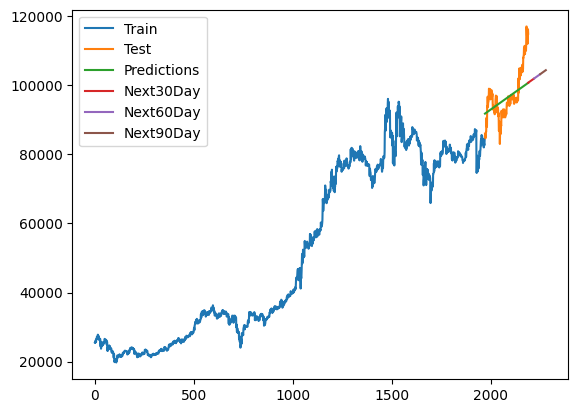
\includegraphics[width=\textwidth]{Figure/FPT/linear91.png}
        \caption{LR with 9:1 ratio}
        \label{fig:image1}
    \end{minipage}
    \hfill
    \begin{minipage}{0.24\textwidth}
        \centering
        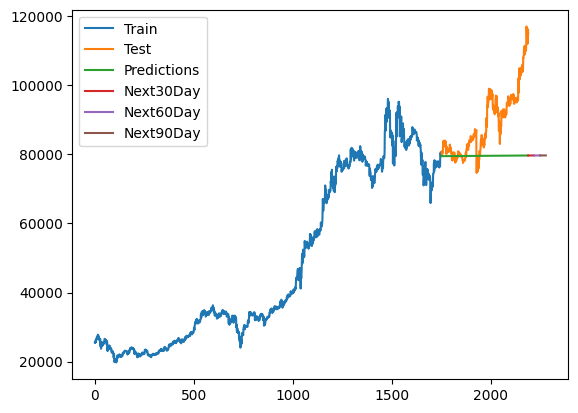
\includegraphics[width=\textwidth]{Figure/FPT/stacking82.png}
        \caption{Stacking with 8:2 ratio}
        \label{fig:image2}
    \end{minipage}
\end{figure}


\begin{figure}[H]
    \centering
    \begin{minipage}{0.24\textwidth}
        \centering
        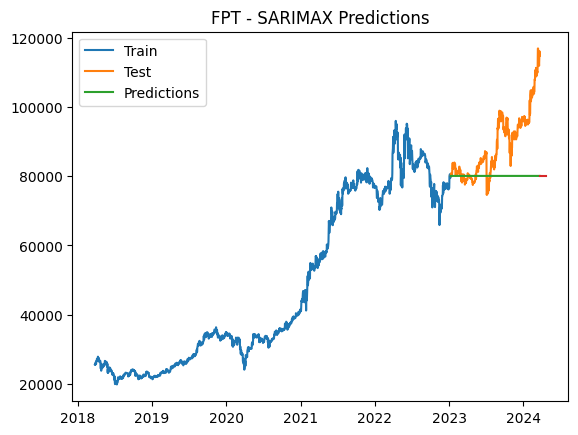
\includegraphics[width=\textwidth]{Figure/FPT/sarimax82.png}
        \caption{Sarimax with 8:2 ratio}
        \label{fig:image1}
    \end{minipage}
    \hfill
    \begin{minipage}{0.24\textwidth}
        \centering
        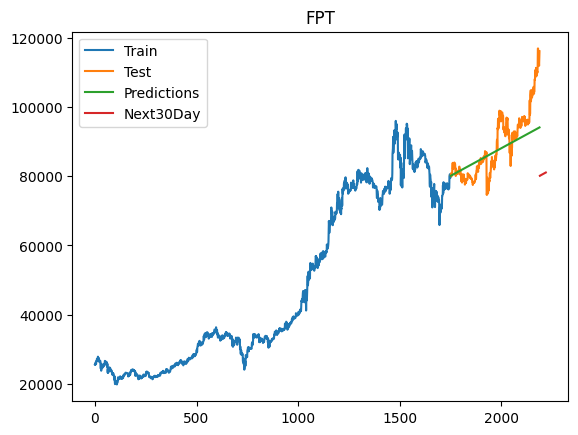
\includegraphics[width=\textwidth]{Figure/FPT/arima82.png}
        \caption{Arima with 8:2 ratio}
        \label{fig:image2}
    \end{minipage}
\end{figure}


\begin{figure}[H]
    \centering
    \begin{minipage}{0.24\textwidth}
        \centering
        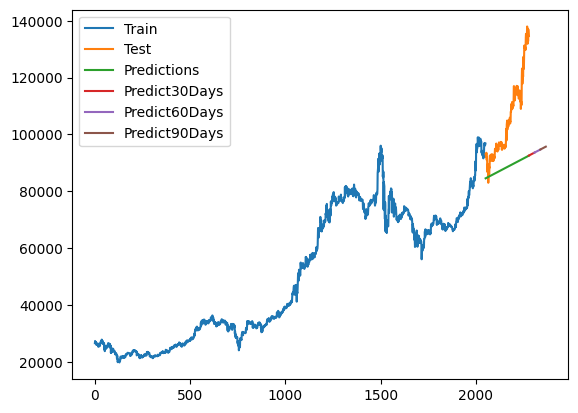
\includegraphics[width=\textwidth]{Figure/FPT/boosting91.png}
        \caption{Boosting with 9:1 ratio}
        \label{fig:image1}
    \end{minipage}
    \hfill
    \begin{minipage}{0.24\textwidth}
        \centering
        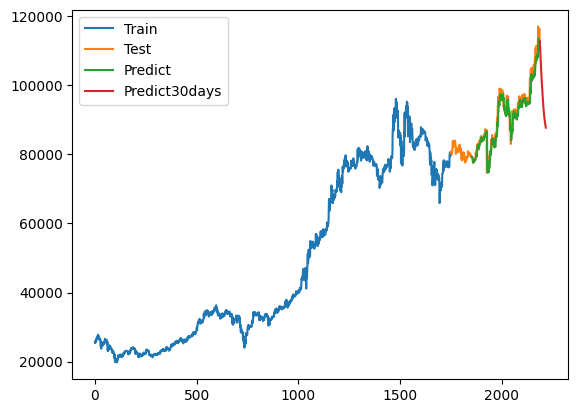
\includegraphics[width=\textwidth]{Figure/FPT/rnn82.png}
        \caption{RNN with 8:2 ratio}
        \label{fig:image2}
    \end{minipage}
\end{figure}


\begin{figure}[H]
    \centering
    \begin{minipage}{0.24\textwidth}
        \centering
        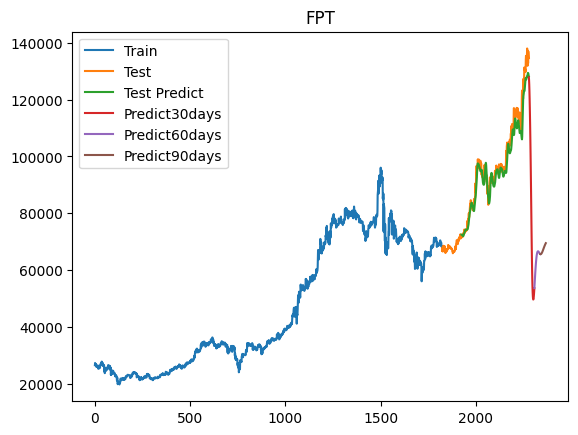
\includegraphics[width=\textwidth]{Figure/FPT/lstm82.png}
        \caption{LSTM with 8:2 ratio}
        \label{fig:image1}
    \end{minipage}
    \hfill
    \begin{minipage}{0.24\textwidth}
        \centering
        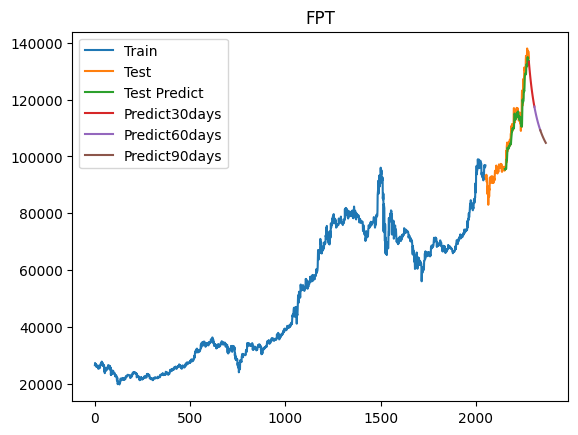
\includegraphics[width=\textwidth]{Figure/FPT/gru91.png}
        \caption{GRU with 9:1 ratio}
        \label{fig:image2}
    \end{minipage}
\end{figure}

\begin{figure}[H]
    \centering
    \begin{minipage}{0.24\textwidth}
        \centering
        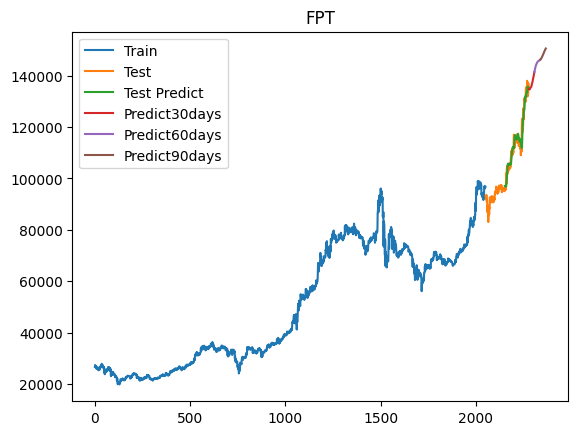
\includegraphics[width=\textwidth]{Figure/FPT/cnnlstm91.png}
        \caption{CNN-LSTM with 9:1 ratio}
        \label{fig:image1}
    \end{minipage}
    \hfill
    \begin{minipage}{0.24\textwidth}
        \centering
        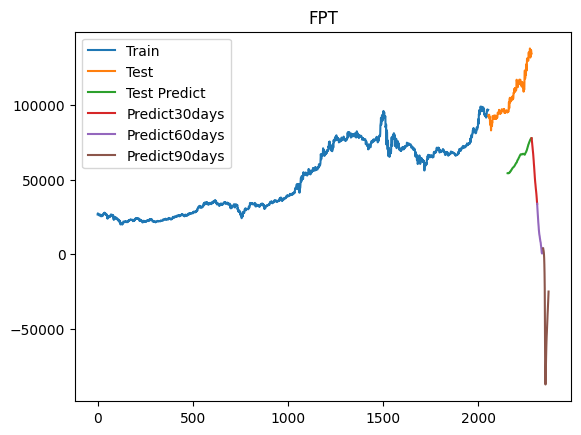
\includegraphics[width=\textwidth]{Figure/FPT/resnet91.png}
        \caption{ResNet with 8:2 ratio}
        \label{fig:image2}
    \end{minipage}
\end{figure}


\subsubsection{CMG DATASET}  {Visualization of CMG dataset}

\begin{figure}[H]
    \centering
    \begin{minipage}{0.24\textwidth}
        \centering
        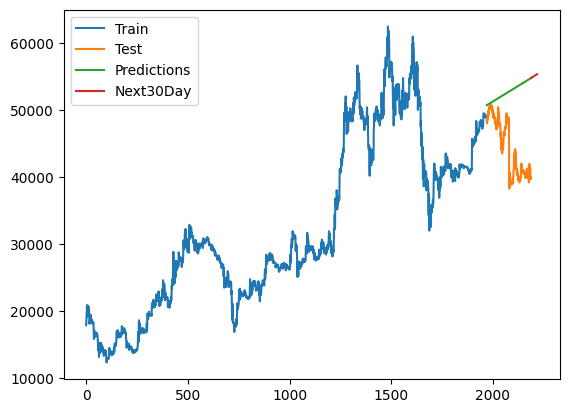
\includegraphics[width=\textwidth]{Figure/CMG/linear91.png}
        \caption{LR with 9:1 ratio}
        \label{fig:image1}
    \end{minipage}
    \hfill
    \begin{minipage}{0.24\textwidth}
        \centering
        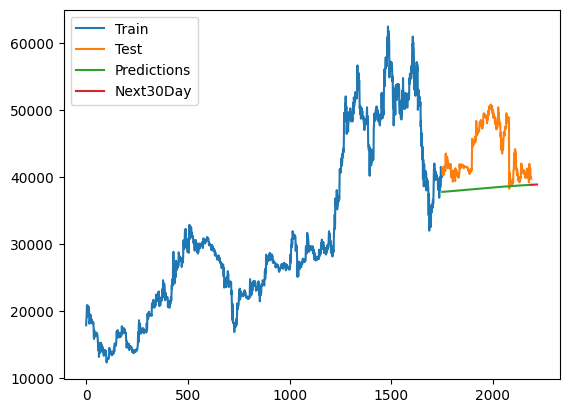
\includegraphics[width=\textwidth]{Figure/CMG/stacking82.png}
        \caption{Stacking with 8:2 ratio}
        \label{fig:image2}
    \end{minipage}
\end{figure}


\begin{figure}[H]
    \centering
    \begin{minipage}{0.24\textwidth}
        \centering
        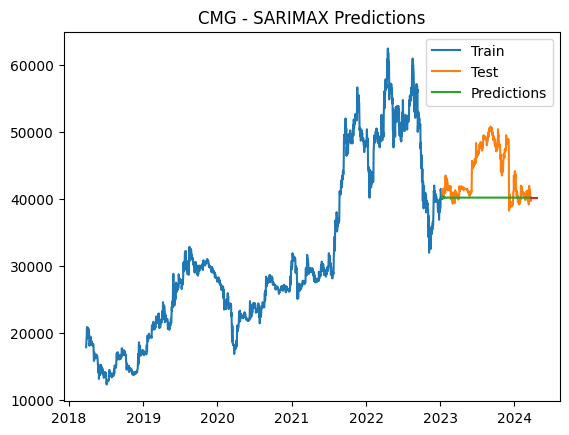
\includegraphics[width=\textwidth]{Figure/CMG/sarimax82.png}
        \caption{Sarimax with 8:2 ratio}
        \label{fig:image1}
    \end{minipage}
    \hfill
    \begin{minipage}{0.24\textwidth}
        \centering
        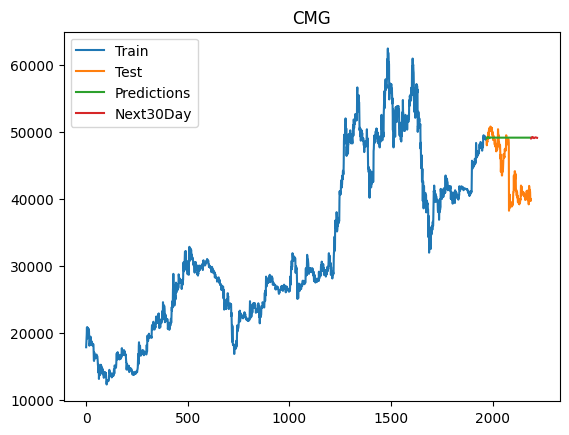
\includegraphics[width=\textwidth]{Figure/CMG/arima82.png}
        \caption{Arima with 8:2 ratio}
        \label{fig:image2}
    \end{minipage}
\end{figure}


\begin{figure}[H]
    \centering
    \begin{minipage}{0.24\textwidth}
        \centering
        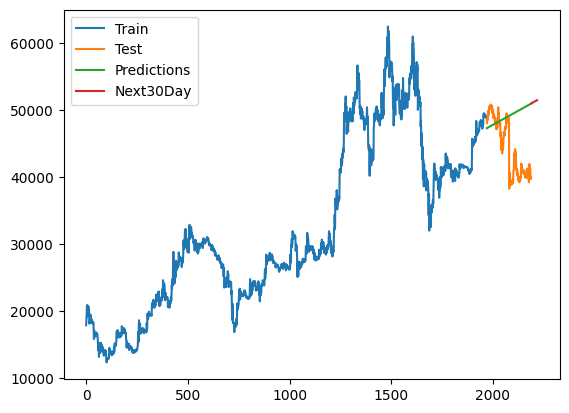
\includegraphics[width=\textwidth]{Figure/CMG/boosting91.png}
        \caption{Boosting with 9:1 ratio}
        \label{fig:image1}
    \end{minipage}
    \hfill
    \begin{minipage}{0.24\textwidth}
        \centering
        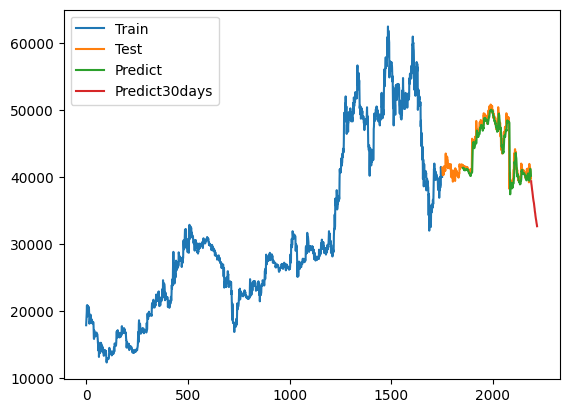
\includegraphics[width=\textwidth]{Figure/CMG/rnn82.png}
        \caption{RNN with 8:2 ratio}
        \label{fig:image2}
    \end{minipage}
\end{figure}


\begin{figure}[H]
    \centering
    \begin{minipage}{0.24\textwidth}
        \centering
        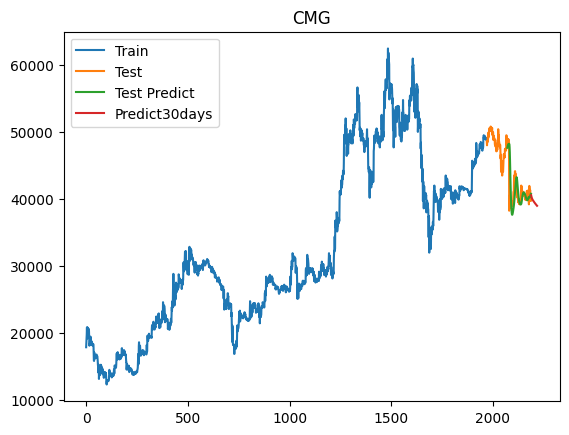
\includegraphics[width=\textwidth]{Figure/CMG/lstm91.png}
        \caption{LSTM with 9:1 ratio}
        \label{fig:image1}
    \end{minipage}
    \hfill
    \begin{minipage}{0.24\textwidth}
        \centering
        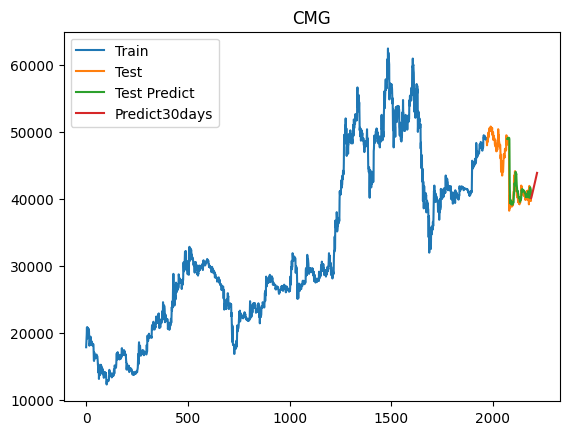
\includegraphics[width=\textwidth]{Figure/CMG/gru91.png}
        \caption{GRU with 9:1 ratio}
        \label{fig:image2}
    \end{minipage}
\end{figure}

\begin{figure}[H]
    \centering
    \begin{minipage}{0.24\textwidth}
        \centering
        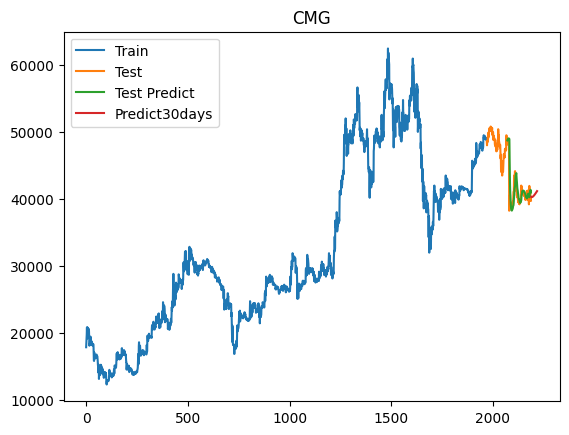
\includegraphics[width=\textwidth]{Figure/CMG/cnnlstm91.png}
        \caption{CNN-LSTM with 9:1 ratio}
        \label{fig:image1}
    \end{minipage}
    \hfill
    \begin{minipage}{0.24\textwidth}
        \centering
        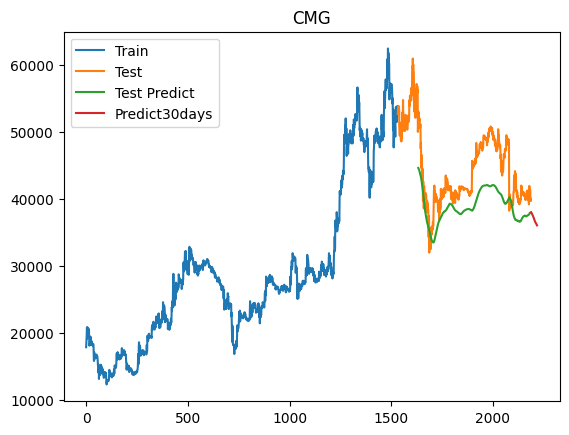
\includegraphics[width=\textwidth]{Figure/CMG/resnet73.png}
        \caption{ResNet with 7:3 ratio}
        \label{fig:image2}
    \end{minipage}
\end{figure}


\subsubsection{ELC DATASET}  {Visualization of ELC dataset}

\begin{figure}[H]
    \centering
    \begin{minipage}{0.24\textwidth}
        \centering
        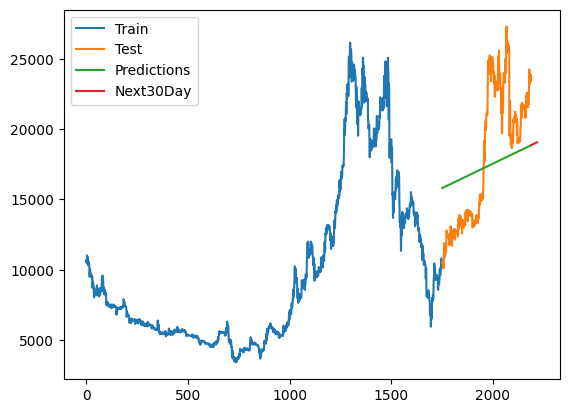
\includegraphics[width=\textwidth]{Figure/ELC/linear82.png}
        \caption{LR with 8:2 ratio}
        \label{fig:image1}
    \end{minipage}
    \hfill
    \begin{minipage}{0.24\textwidth}
        \centering
        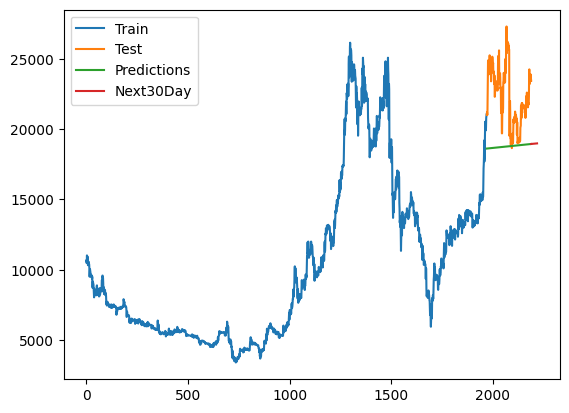
\includegraphics[width=\textwidth]{Figure/ELC/stacking91.png}
        \caption{Stacking with 9:1 ratio}
        \label{fig:image2}
    \end{minipage}
\end{figure}


\begin{figure}[H]
    \centering
    \begin{minipage}{0.24\textwidth}
        \centering
        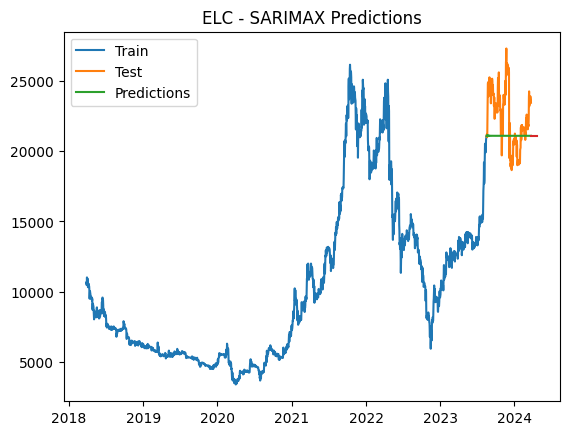
\includegraphics[width=\textwidth]{Figure/ELC/sarimax91.png}
        \caption{Sarimax with 9:1 ratio}
        \label{fig:image1}
    \end{minipage}
    \hfill
    \begin{minipage}{0.24\textwidth}
        \centering
        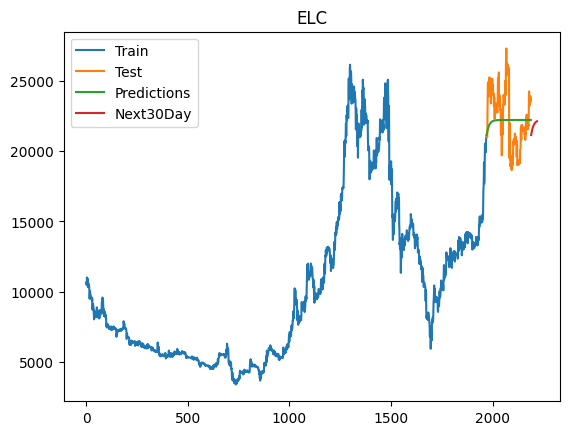
\includegraphics[width=\textwidth]{Figure/ELC/arima91.png}
        \caption{Arima with 9:1 ratio}
        \label{fig:image2}
    \end{minipage}
\end{figure}


\begin{figure}[H]
    \centering
    \begin{minipage}{0.24\textwidth}
        \centering
        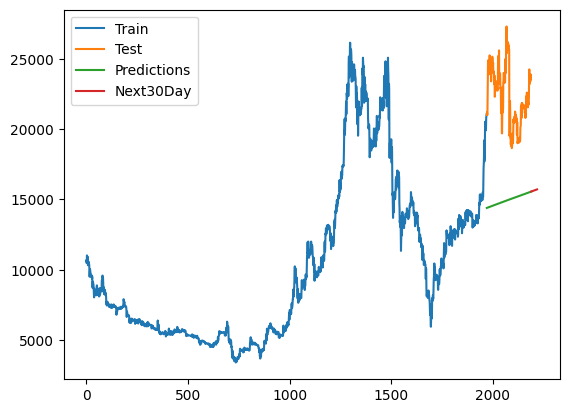
\includegraphics[width=\textwidth]{Figure/ELC/boosting91.png}
        \caption{Boosting with 9:1 ratio}
        \label{fig:image1}
    \end{minipage}
    \hfill
    \begin{minipage}{0.24\textwidth}
        \centering
        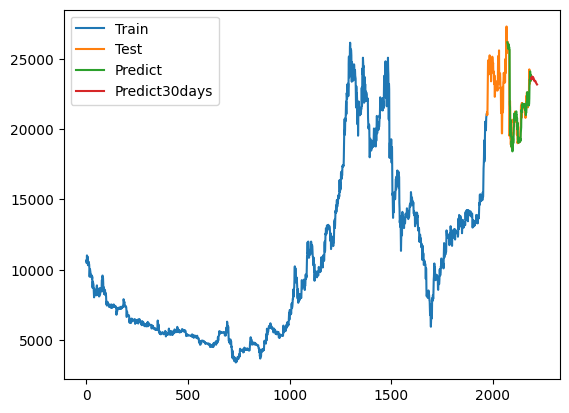
\includegraphics[width=\textwidth]{Figure/ELC/rnn91.png}
        \caption{RNN with 9:1 ratio}
        \label{fig:image2}
    \end{minipage}
\end{figure}


\begin{figure}[H]
    \centering
    \begin{minipage}{0.24\textwidth}
        \centering
        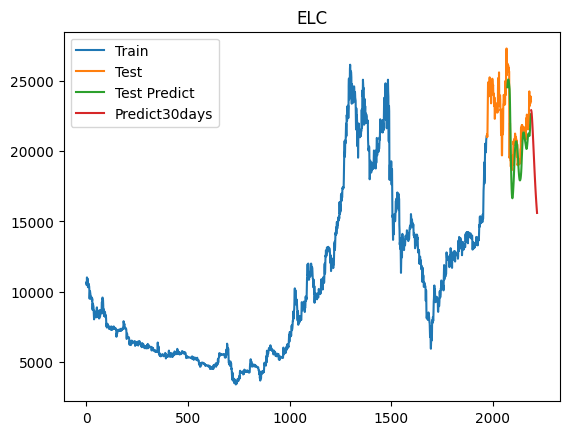
\includegraphics[width=\textwidth]{Figure/ELC/lstm91.png}
        \caption{LSTM with 9:1 ratio}
        \label{fig:image1}
    \end{minipage}
    \hfill
    \begin{minipage}{0.24\textwidth}
        \centering
        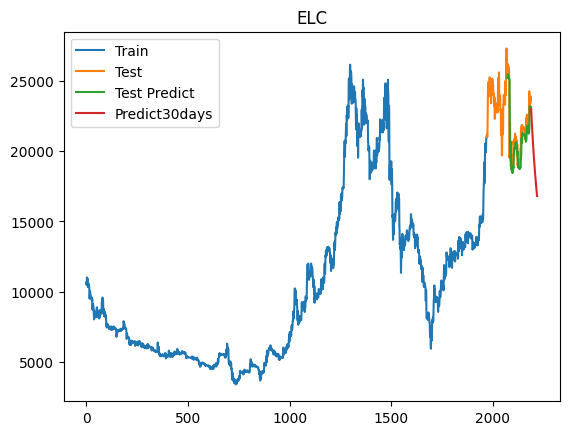
\includegraphics[width=\textwidth]{Figure/ELC/gru91.png}
        \caption{GRU with 9:1 ratio}
        \label{fig:image2}
    \end{minipage}
\end{figure}

\begin{figure}[H]
    \centering
    \begin{minipage}{0.24\textwidth}
        \centering
        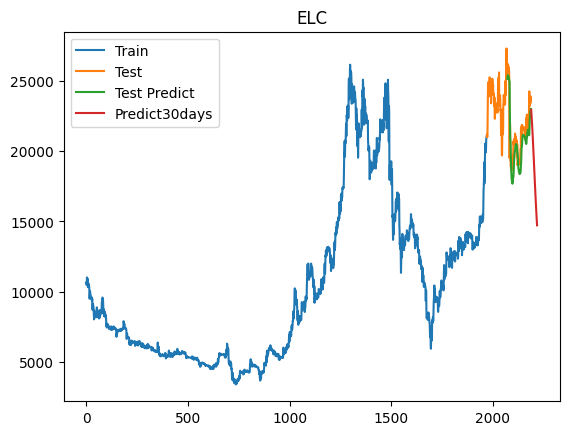
\includegraphics[width=\textwidth]{Figure/ELC/cnnlstm91.png}
        \caption{CNN-LSTM with 9:1 ratio}
        \label{fig:image1}
    \end{minipage}
    \hfill
    \begin{minipage}{0.24\textwidth}
        \centering
        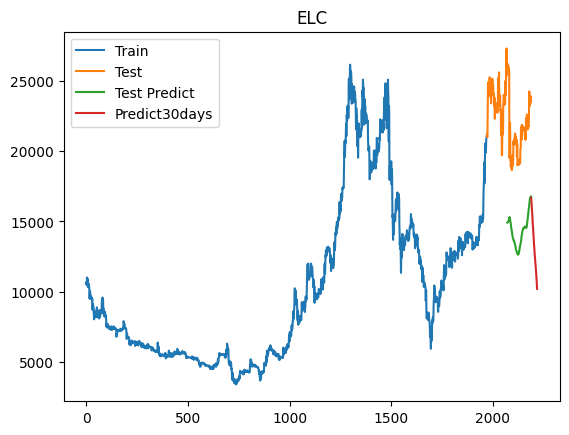
\includegraphics[width=\textwidth]{Figure/ELC/resnet91.png}
        \caption{ResNet with 9:1 ratio}
        \label{fig:image2}
    \end{minipage}
\end{figure}

\section{CONCLUSION}
\subsection{SUMMARY}
In this study, we conducted a comprehensive comparative analysis of ten models—Linear Regression, ARIMA, RNN, GRU, LSTM, SARIMAX, Boosting Model, Stacking Model, ResNet, and CNN-LSTM—using three Vietnamese tech stock market datasets: ELC, CMG, and FPT. Our findings revealed that while traditional models like Linear Regression and ARIMA provided baseline results, they were outperformed by more sophisticated methods. RNN, GRU, and LSTM showed significant improvements, with LSTM being particularly effective in capturing long-term dependencies. SARIMAX demonstrated the benefits of incorporating exogenous variables, and ensemble methods like the Stacking Model displayed robust performance. Among deep learning models, ResNet and CNN-LSTM achieved the highest accuracy, with CNN-LSTM excelling by effectively combining spatial and temporal features. Thus, while traditional models are useful for baseline comparisons, advanced deep learning techniques, particularly CNN-LSTM and LSTM, are more reliable and accurate for predicting stock prices in the Vietnamese tech market. 

\subsection{CHALLENGES AND FUTURE DIRECTION}
Addressing the optimal parameter selection for each model proved to be a time-consuming and computationally demanding task, particularly for intricate models such as RNN, GRU, LSTM, and CNN-LSTM. The datasets utilized in the study, namely ELC, CMG, and FPT, were constrained by their limited attributes, which in turn limited the predictive accuracy of the models. The deficiency in attributes underscored the necessity for more comprehensive datasets encompassing a wider array of features pertinent to stock price prediction. Future endeavors should prioritize the augmentation of datasets with diverse attributes and the exploration of advanced feature engineering techniques to bolster model performance. By leveraging richer datasets and innovative methodologies, the predictive capabilities of stock price prediction models can be significantly enhanced.



\bibliographystyle{ieeetr}
\bibliography{ref}

\end{document}
